\documentclass[border=3pt]{standalone}
% Shared preamble for the standalone figures of qurl_explained.tex.
% Build a figure from this folder:   tectonic fig_<name>.tex
% Colours: blue = full precision (FP), orange = 8-bit.
\usepackage[T1]{fontenc}
\usepackage{lmodern}
\usepackage{amsmath,amssymb}
\usepackage[dvipsnames]{xcolor}
\usepackage{tikz}
\usetikzlibrary{positioning,arrows.meta,calc,decorations.pathreplacing}
\usepackage{pgfplots}
\pgfplotsset{compat=1.17}
\colorlet{fp}{RoyalBlue}
\colorlet{qb}{BurntOrange}
\colorlet{good}{ForestGreen}
\colorlet{bad}{BrickRed}
\newcommand{\pold}{\pi_{\mathrm{old}}}
\newcommand{\thold}{\theta_{\mathrm{old}}}
\newcommand{\qthold}{\hat\theta_{\mathrm{old}}}
\tikzset{
  box/.style={draw, rounded corners=3pt, align=center, inner sep=4pt, font=\small},
  arr/.style={-{Stealth[length=2.2mm]}, thick},
  lab/.style={font=\footnotesize, align=center},
}
\pgfplotsset{
  small axes/.style={
    tick label style={font=\footnotesize}, label style={font=\footnotesize},
    title style={font=\small}, every axis plot/.append style={line join=round}},
}

\begin{document}
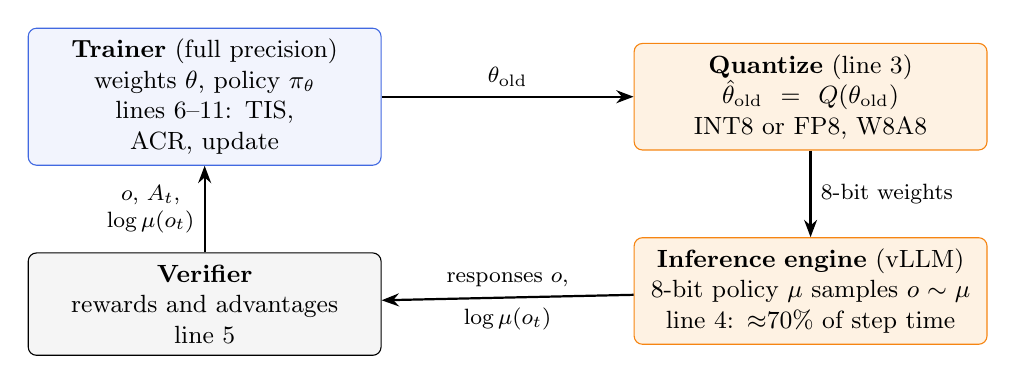
\begin{tikzpicture}[b/.style={box, text width=4.2cm, minimum height=1.3cm}]
\node[b, draw=fp, fill=fp!7] (train) {\textbf{Trainer} (full precision)\\ weights $\theta$, policy $\pi_\theta$\\ lines 6--11: TIS, ACR, update};
\node[b, draw=qb, fill=qb!9, right=3.2cm of train] (quant) {\textbf{Quantize} (line 3)\\ $\qthold=Q(\thold)$\\ INT8 or FP8, W8A8};
\node[b, draw=qb, fill=qb!9, below=1.1cm of quant] (engine) {\textbf{Inference engine} (vLLM)\\ 8-bit policy $\mu$ samples $o\sim\mu$\\ line 4: ${\approx}70\%$ of step time};
\node[b, fill=black!4, below=1.1cm of train] (verify) {\textbf{Verifier}\\ rewards and advantages\\ line 5};
\draw[arr] (train) -- node[lab, above] {$\thold$} (quant);
\draw[arr] (quant) -- node[lab, right] {8-bit weights} (engine);
\draw[arr] (engine) -- node[lab, above] {responses $o$,} node[lab, below] {$\log\mu(o_t)$} (verify);
\draw[arr] (verify) -- node[lab, left] {$o$, $A_t$,\\ $\log\mu(o_t)$} (train);
\end{tikzpicture}
\end{document}
